\section{Evidence-Aligned Medical Representation Learning}
\subsection{HybridMED: aligning report structure and images}
Reports describe image findings at different semantic levels. HybridMED \citep{hybridmed} aligns global image representations with report impressions and token-level visual representations with findings. Its generation decoder learns captioning and summarization proxy tasks, with knowledge distilled from summarization to captioning. This arrangement draws on the complementary roles of descriptive observations and higher-level clinical summaries. Pretraining uses MIMIC-CXR, with approximately 135,000 image--report pairs after preprocessing from approximately 232,000 images and 367,000 reports.

HybridMED reports zero-shot RSNA Pneumonia accuracy of 0.800 and CheXpert accuracy of 0.448, as well as fully supervised AUCs of 0.902 on RSNA and 0.893 on CheXpert. The generation branches share self-attention and feed-forward architecture; this supports an architectural parameter-efficiency argument without an explicit parameter count or FLOP comparison. Sharing allows the proxy tasks to exchange representational structure while avoiding a separate full decoder for each task.

Hanqi Jiang is first author and lead of the ECCV Workshop 2024 work. The study shows how naturally occurring report organization can supervise alignment without requiring a separate pixel-level annotation for each example.

\subsection{EGMA: gaze-guided multimodal alignment}
EGMA \citep{egma} uses synchronously collected radiologist gaze to guide alignment between medical images and text. Gaze offers an auxiliary clinical signal about where attention was allocated during reading. It can encourage the representation to capture image regions associated with report content instead of relying only on a global image--text match. The work evaluates classification and image--text retrieval across four medical datasets and reports competitive classification and image--text retrieval, with cross-dataset generalization.
Figure~\ref{fig:egma_framework} shows the alignment pipeline.
\begin{figure}[htbp]\centering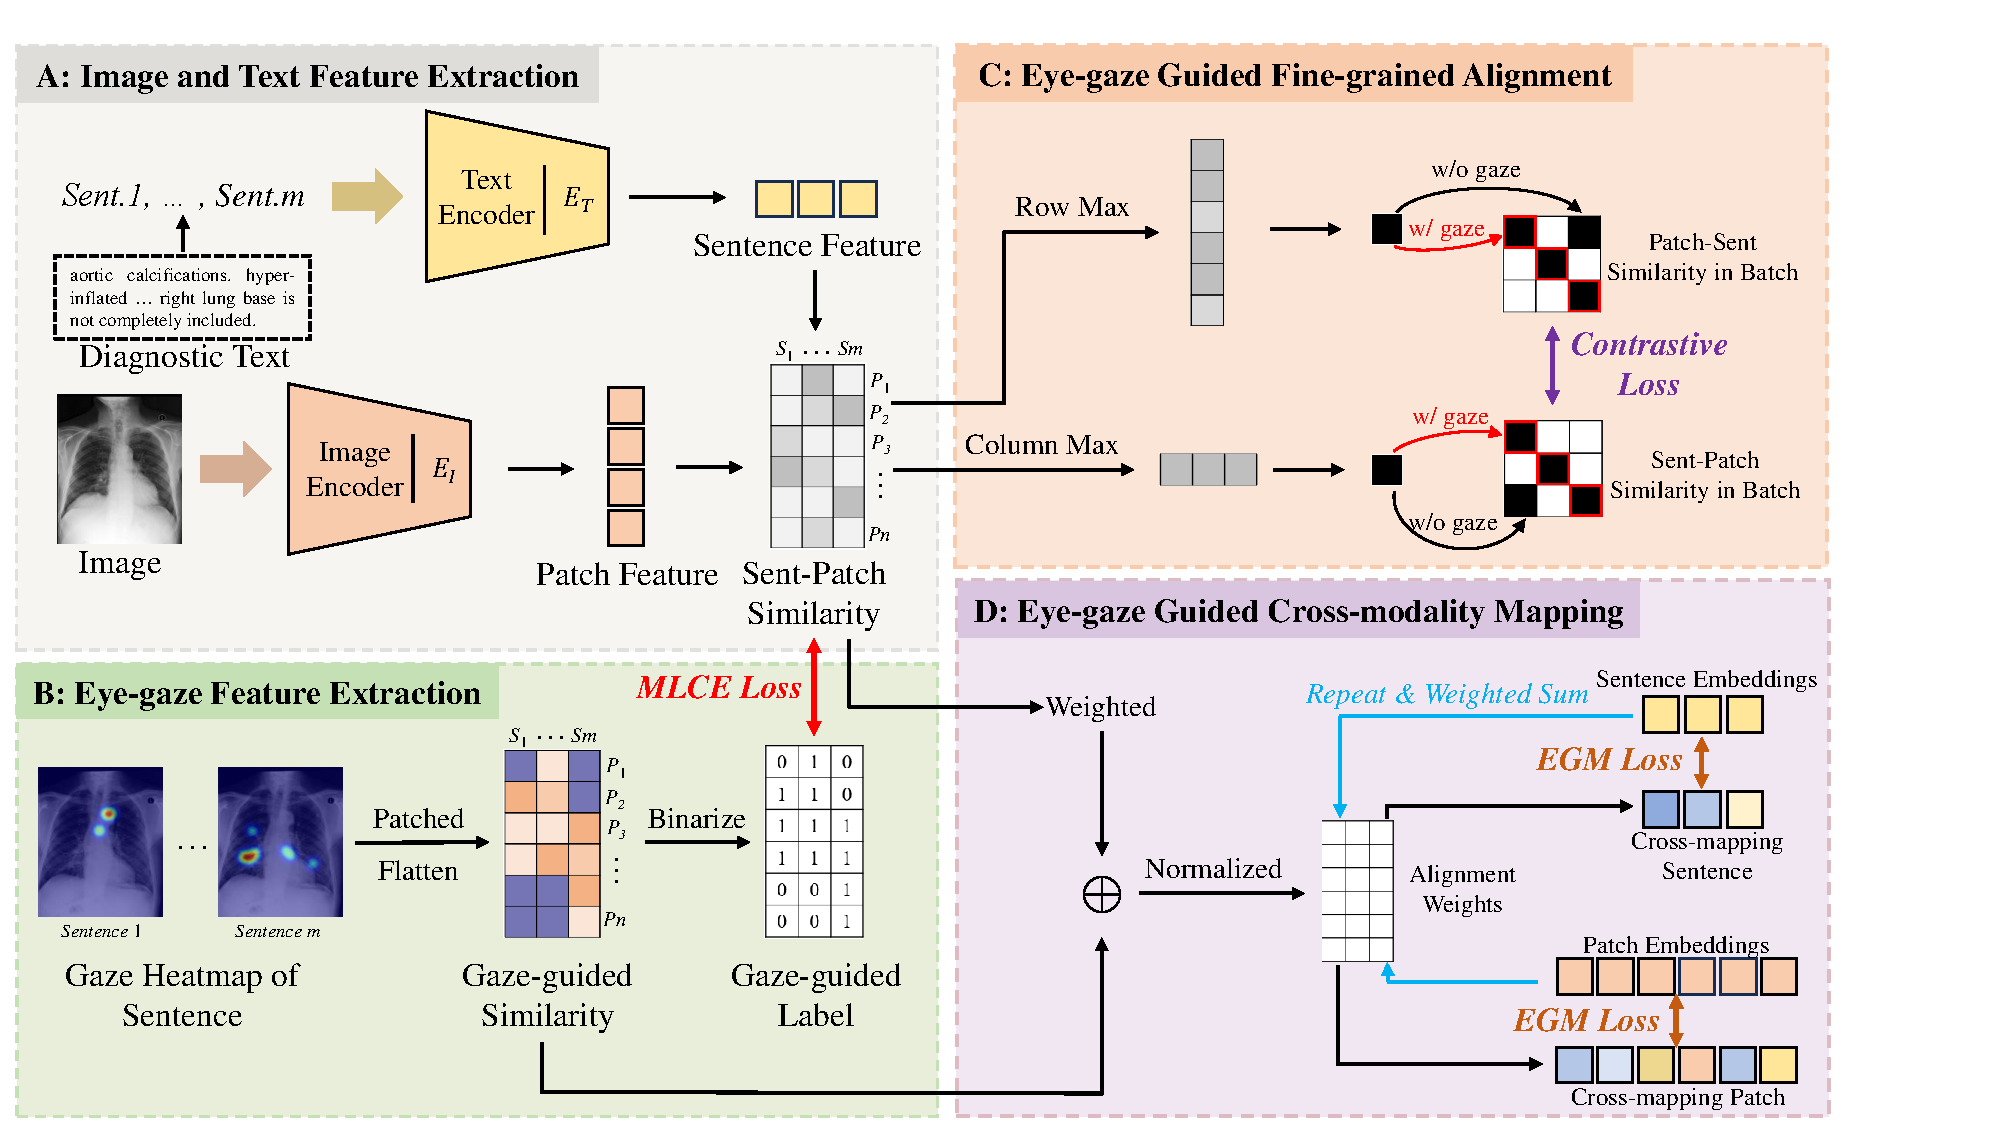
\includegraphics[width=\textwidth,height=.30\textheight,keepaspectratio]{figures/egma_framework.pdf}\caption{EGMA first encodes image--text pairs in Part A to obtain patch and sentence features and an instance similarity matrix. Part B combines eye gaze, images, and audio transcripts to produce an attention heatmap and gaze-guided similarity and label matrices. Part C uses the label matrix to guide fine-grained alignment of patches and sentences. Part D uses the gaze-guided similarity matrix and mapped features for cross-modality mapping, producing cross-mapped features and an alignment loss. Adapted from EGMA Fig. 2. Source: EGMA \citep{egma}.}\label{fig:egma_framework}\end{figure}

By varying the amount of gaze supervision, the study reports that even a small amount can assist multimodal pretraining. This is a qualitative auxiliary-data efficiency result; gaze collection requires clinical expertise and equipment. Hanqi Jiang is second author; Tianming Liu and Xiang Li were corresponding authors of the NeurIPS 2024 work.

\subsection{EG-SpikeFormer: gaze and event-driven computation}
EG-SpikeFormer \citep{egspike} combines an eye-gaze-guided Transformer with spiking neural network computation for medical image analysis. Gaze can help steer learning toward clinically relevant image regions, addressing shortcut reliance, while spikes offer an event-driven computational substrate. The alignment and computational choices work together but answer different questions: gaze concerns relevance, and spiking concerns the operations needed to process information.

The reported Ours-T2 and Ours-T4 energy values are 26.7 and 52.4 mJ, compared with 81.0 mJ for ViT and 56.6 mJ for EfficientNet under the paper's comparison. Ours-T4 reaches 94.32\% accuracy and 93.00\% AUC on INbreast, and 88.28\% accuracy on SIIM-ACR. The table also reports lower energy for several other models, including 19.0 mJ for ResNet-50, 13.8 mJ for Swin-T, and 10.2 mJ for MS-Res-SNN. Thus the finding is an energy--accuracy trade-off, not a claim of minimum energy. Comparisons depend on the paper's energy accounting and should not be read as measured energy for arbitrary clinical hardware.

Hanqi Jiang is co-first author with Yi Pan, with equal contribution, on the ISBI 2025 Oral paper. The result illustrates how an explicitly medical alignment objective and a resource-aware architecture can be evaluated together while preserving the distinction between clinical relevance and computational cost.

\subsection{Synthesis}
Report structure and gaze provide complementary supervision: reports express semantic relationships, while gaze supplies a signal tied to visual reading. HybridMED emphasizes shared parameters, EGMA the utility of auxiliary data, and EG-SpikeFormer the energy cost of computation. These are alignment results rather than proofs of evidence use at generation time. The subsequent sections make the behavior of a model under selective perception and failed evidence directly testable.
